% Options for packages loaded elsewhere
\PassOptionsToPackage{unicode}{hyperref}
\PassOptionsToPackage{hyphens}{url}
%
\documentclass[
]{article}
\usepackage{amsmath,amssymb}
\usepackage{iftex}
\ifPDFTeX
  \usepackage[T1]{fontenc}
  \usepackage[utf8]{inputenc}
  \usepackage{textcomp} % provide euro and other symbols
\else % if luatex or xetex
  \usepackage{unicode-math} % this also loads fontspec
  \defaultfontfeatures{Scale=MatchLowercase}
  \defaultfontfeatures[\rmfamily]{Ligatures=TeX,Scale=1}
\fi
\usepackage{lmodern}
\ifPDFTeX\else
  % xetex/luatex font selection
\fi
% Use upquote if available, for straight quotes in verbatim environments
\IfFileExists{upquote.sty}{\usepackage{upquote}}{}
\IfFileExists{microtype.sty}{% use microtype if available
  \usepackage[]{microtype}
  \UseMicrotypeSet[protrusion]{basicmath} % disable protrusion for tt fonts
}{}
\makeatletter
\@ifundefined{KOMAClassName}{% if non-KOMA class
  \IfFileExists{parskip.sty}{%
    \usepackage{parskip}
  }{% else
    \setlength{\parindent}{0pt}
    \setlength{\parskip}{6pt plus 2pt minus 1pt}}
}{% if KOMA class
  \KOMAoptions{parskip=half}}
\makeatother
\usepackage{xcolor}
\usepackage[margin=1in]{geometry}
\usepackage{color}
\usepackage{fancyvrb}
\newcommand{\VerbBar}{|}
\newcommand{\VERB}{\Verb[commandchars=\\\{\}]}
\DefineVerbatimEnvironment{Highlighting}{Verbatim}{commandchars=\\\{\}}
% Add ',fontsize=\small' for more characters per line
\usepackage{framed}
\definecolor{shadecolor}{RGB}{248,248,248}
\newenvironment{Shaded}{\begin{snugshade}}{\end{snugshade}}
\newcommand{\AlertTok}[1]{\textcolor[rgb]{0.94,0.16,0.16}{#1}}
\newcommand{\AnnotationTok}[1]{\textcolor[rgb]{0.56,0.35,0.01}{\textbf{\textit{#1}}}}
\newcommand{\AttributeTok}[1]{\textcolor[rgb]{0.13,0.29,0.53}{#1}}
\newcommand{\BaseNTok}[1]{\textcolor[rgb]{0.00,0.00,0.81}{#1}}
\newcommand{\BuiltInTok}[1]{#1}
\newcommand{\CharTok}[1]{\textcolor[rgb]{0.31,0.60,0.02}{#1}}
\newcommand{\CommentTok}[1]{\textcolor[rgb]{0.56,0.35,0.01}{\textit{#1}}}
\newcommand{\CommentVarTok}[1]{\textcolor[rgb]{0.56,0.35,0.01}{\textbf{\textit{#1}}}}
\newcommand{\ConstantTok}[1]{\textcolor[rgb]{0.56,0.35,0.01}{#1}}
\newcommand{\ControlFlowTok}[1]{\textcolor[rgb]{0.13,0.29,0.53}{\textbf{#1}}}
\newcommand{\DataTypeTok}[1]{\textcolor[rgb]{0.13,0.29,0.53}{#1}}
\newcommand{\DecValTok}[1]{\textcolor[rgb]{0.00,0.00,0.81}{#1}}
\newcommand{\DocumentationTok}[1]{\textcolor[rgb]{0.56,0.35,0.01}{\textbf{\textit{#1}}}}
\newcommand{\ErrorTok}[1]{\textcolor[rgb]{0.64,0.00,0.00}{\textbf{#1}}}
\newcommand{\ExtensionTok}[1]{#1}
\newcommand{\FloatTok}[1]{\textcolor[rgb]{0.00,0.00,0.81}{#1}}
\newcommand{\FunctionTok}[1]{\textcolor[rgb]{0.13,0.29,0.53}{\textbf{#1}}}
\newcommand{\ImportTok}[1]{#1}
\newcommand{\InformationTok}[1]{\textcolor[rgb]{0.56,0.35,0.01}{\textbf{\textit{#1}}}}
\newcommand{\KeywordTok}[1]{\textcolor[rgb]{0.13,0.29,0.53}{\textbf{#1}}}
\newcommand{\NormalTok}[1]{#1}
\newcommand{\OperatorTok}[1]{\textcolor[rgb]{0.81,0.36,0.00}{\textbf{#1}}}
\newcommand{\OtherTok}[1]{\textcolor[rgb]{0.56,0.35,0.01}{#1}}
\newcommand{\PreprocessorTok}[1]{\textcolor[rgb]{0.56,0.35,0.01}{\textit{#1}}}
\newcommand{\RegionMarkerTok}[1]{#1}
\newcommand{\SpecialCharTok}[1]{\textcolor[rgb]{0.81,0.36,0.00}{\textbf{#1}}}
\newcommand{\SpecialStringTok}[1]{\textcolor[rgb]{0.31,0.60,0.02}{#1}}
\newcommand{\StringTok}[1]{\textcolor[rgb]{0.31,0.60,0.02}{#1}}
\newcommand{\VariableTok}[1]{\textcolor[rgb]{0.00,0.00,0.00}{#1}}
\newcommand{\VerbatimStringTok}[1]{\textcolor[rgb]{0.31,0.60,0.02}{#1}}
\newcommand{\WarningTok}[1]{\textcolor[rgb]{0.56,0.35,0.01}{\textbf{\textit{#1}}}}
\usepackage{graphicx}
\makeatletter
\def\maxwidth{\ifdim\Gin@nat@width>\linewidth\linewidth\else\Gin@nat@width\fi}
\def\maxheight{\ifdim\Gin@nat@height>\textheight\textheight\else\Gin@nat@height\fi}
\makeatother
% Scale images if necessary, so that they will not overflow the page
% margins by default, and it is still possible to overwrite the defaults
% using explicit options in \includegraphics[width, height, ...]{}
\setkeys{Gin}{width=\maxwidth,height=\maxheight,keepaspectratio}
% Set default figure placement to htbp
\makeatletter
\def\fps@figure{htbp}
\makeatother
\setlength{\emergencystretch}{3em} % prevent overfull lines
\providecommand{\tightlist}{%
  \setlength{\itemsep}{0pt}\setlength{\parskip}{0pt}}
\setcounter{secnumdepth}{-\maxdimen} % remove section numbering
\ifLuaTeX
  \usepackage{selnolig}  % disable illegal ligatures
\fi
\IfFileExists{bookmark.sty}{\usepackage{bookmark}}{\usepackage{hyperref}}
\IfFileExists{xurl.sty}{\usepackage{xurl}}{} % add URL line breaks if available
\urlstyle{same}
\hypersetup{
  pdftitle={Sage Babish and Victoria Peechatt},
  pdfauthor={BIOL792 Final Project},
  hidelinks,
  pdfcreator={LaTeX via pandoc}}

\title{Sage Babish and Victoria Peechatt}
\author{BIOL792 Final Project}
\date{2023-12-06}

\begin{document}
\maketitle

\hypertarget{numpy-pandas-data-cleaning-and-visualization}{%
\section{NumPy, pandas, data cleaning and
visualization}\label{numpy-pandas-data-cleaning-and-visualization}}

For this project, we used Pandas and NumPy to clean and extract data
from our datasets. We both have rather different study systems and
datasets, but we were able to make a couple programs useful for both of
us (maybe with a little tweaking). Here, we present our problems and the
steps we followed to address those problems, largely in the form of
python code. We also present our next steps, both with our data and what
else we hope to learn to do with NumPy, pandas, and python.

\hypertarget{sage-has-multiple-peoples-specimen-catalogs-data-on-snake-ttx-resistance-in-multiple-formats-and-a-host-of-other-unorganized-files-to-extract-data-from.}{%
\subsection{Sage has multiple people's specimen catalogs, data on snake
TTX resistance in multiple formats, and a host of other unorganized
files to extract data
from.}\label{sage-has-multiple-peoples-specimen-catalogs-data-on-snake-ttx-resistance-in-multiple-formats-and-a-host-of-other-unorganized-files-to-extract-data-from.}}

I needed two different sets of information from these data sets. First,
which specimens collected by our lab and our collaborators were from my
study area, and did we have tissue samples, sequencing data, or
phenotypes for them? Second, which specimens had phenotypes, base
speeds, and at least one out of SVL, mass, and tail length? The first
information was used to figure out how many tissue/genetic samples we
already had and how many new ones would need to be requested from
museums or captured in the field and phenotyped. The second set will be
used to model the effects of mass, size, body condition, and TTX
resistance on base speed in an attempt to observe a trade-off between
resistance and muscle function.

\hypertarget{part-1-catalog-searches}{%
\subsubsection{Part 1: Catalog Searches}\label{part-1-catalog-searches}}

My first steps for this project were parsing through several specimen
collection catalogs and extracting specimens based on increasingly
specific qualifications. This is what the heads of some of those
catalogs look like, to give an idea of what I was working with:

\begin{verbatim}
##   CollPreNo CollNo CollPre      Genus           Sp        Ssp      County
## 1  CRF 0001      1     CRF Thamnophis      elegans terrestris    Alameda 
## 2  CRF 0002      2     CRF  Pituophis melanoleucus  catenifer Stanislaus 
## 3  CRF 0003      3     CRF     Lanius ludovicianus                       
## 4  CRF 0004      4     CRF                                               
## 5  CRF 0005      5     CRF                                               
## 6  CRF 0006      6     CRF                                               
##        State Latitude Longitude  DateColl Sex Remarks Stage
## 1 California                    20-Mar-95                  
## 2 California                                               
## 3                                                 DOR      
## 4                                                          
## 5                                                          
## 6                                                          
##                                                                                          Local
## 1 behind Lawerence Hall of Science, off Stadium Way, Berkeley Hills, Berkeley, Alameda Co., CA
## 2                                                                                             
## 3                                                                                             
## 4                                                                                             
## 5                                                                                             
## 6                                                                                             
##        Collector.s. Alt..ID CollSpLocal Tissues Museum CatNo EcoData Country
## 1 C.R. Feldman, HWG                  NA                   NA             USA
## 2                                    NA                   NA             USA
## 3                                    NA                   NA             USA
## 4                                    NA                   NA             USA
## 5                                    NA                   NA             USA
## 6                                    NA                   NA             USA
##      Class OrderSub Family Continent Skel CollDateYear CollDateMonth
## 1 Reptilia                                        1995           Mar
## 2 Reptilia                                          NA              
## 3                                                   NA              
## 4                                                   NA              
## 5                                                   NA              
## 6                                                   NA              
##   CollDateDay       Elev Tiss Pres IdDate Pubs GenBank
## 1          20 ca. 300 ft   NA               NA        
## 2          NA              NA               NA        
## 3          NA              NA               NA        
## 4          NA              NA               NA        
## 5          NA              NA               NA        
## 6          NA              NA               NA
\end{verbatim}

\begin{verbatim}
##           ID             species         locality    county sex capture_date
## 1 "Sneaky 2"       Charina botae                              -             
## 2   "Sneaky"       Charina botae                              -             
## 3        CRF      Charina bottae       Ash Canyon        NV   -             
## 4    CRF2393  Thamnophis elegans McCullough Ranch    Sonoma   F             
## 5    CRF2509      Charina bottae        Lily Lake El Dorado   -             
## 6    CRF2980 Coluber constrictor                       Yolo   -             
##   lab_entry_date SVL.mm._at_lab_entry mass.g._at_lab_entry mass.g._14Oct2017
## 1                                  NA                   NA                NA
## 2                                  NA                   NA                NA
## 3      27-Feb-17                   NA                   27                NA
## 4      12-May-13                   NA                   NA                NA
## 5      27-Jun-14                   NA                   90                NA
## 6      21-Apr-16                   NA                   NA                NA
##   SVL.mm._16April2018 mass.g._16April2018 SVL.mm._before_muscle_exp
## 1                  21                   6                        NA
## 2                  40                  41                        NA
## 3                                                                NA
## 4                77.5                 255                        NA
## 5                   -                   -                        NA
## 6                63.5                  93                        NA
##   mass.g._before_muscle_exp food_type                  Ivermectin_treatment
## 1                        NA                                                
## 2                        NA                                                
## 3                        NA      mice 12-JULY-2017/27-JULY-2017/10-AUG-2017
## 4                        NA           12-JULY-2017/27-JULY-2017/10-AUG-2017
## 5                        NA      mice 12-JULY-2017/27-JULY-2017/10-AUG-2017
## 6                        NA      mice 12-JULY-2017/27-JULY-2017/10-AUG-2017
##                    Notes X50.MAMU genotype
## 1                                         
## 2                                         
## 3                                         
## 4             Socialized                  
## 5 FOUND DEAD 14-DEC-2017                  
## 6
\end{verbatim}

\begin{verbatim}
##   CollPreNo CollNo CollPre       Genus       Sp      Location County State
## 1    KER001      1     KER  Thamnophis  couchii    Deep Creek Fresno    CA
## 2    KER002      2     KER  Thamnophis  couchii    Deep Creek Fresno    CA
## 3    KER003      3     KER Thamnophis  sirtalis    Deep Creek Fresno    CA
## 4    KER004      4     KER Thamnophis   couchii Emerald Pools Nevada    CA
## 5    KER005      5     KER Thamnophis   couchii Emerald Pools Nevada    CA
## 6    KER006      6     KER Thamnophis   couchii Emerald Pools Nevada    CA
##   Latitude Longitude  DateColl TimeColl  MAMU Toxicity..mg.
## 1 36.93379 -119.2463  6/1/2021    12:55    NA            NA
## 2 36.93379 -119.2463  6/1/2021    13:05 60.00            NA
## 3 36.93379 -119.2463  6/2/2021     8:30  4.79            NA
## 4 36.31927 -120.6567 6/10/2021    12:00  1.01            NA
## 5 36.31927 -120.6567 6/10/2021    12:00  1.10            NA
## 6 36.31927 -120.6567 6/10/2021    13:30  0.41            NA
##                            Notes Stage  X X.1 X.2 X.3 X.4 X.5 X.6 X.7 X.8 X.9
## 1 stationary in water when found adult NA  NA  NA  NA  NA  NA  NA  NA  NA  NA
## 2                   on pond edge adult NA  NA  NA  NA  NA  NA  NA  NA  NA  NA
## 3            under rock, flipped       NA  NA  NA  NA  NA  NA  NA  NA  NA  NA
## 4                                      NA  NA  NA  NA  NA  NA  NA  NA  NA  NA
## 5                                      NA  NA  NA  NA  NA  NA  NA  NA  NA  NA
## 6                                      NA  NA  NA  NA  NA  NA  NA  NA  NA  NA
##   X.10 X.11 X.12 X.13 X.14 X.15 X.16 X.17 X.18 X.19 X.20 X.21 X.22
## 1   NA   NA   NA   NA   NA   NA   NA   NA   NA   NA   NA   NA   NA
## 2   NA   NA   NA   NA   NA   NA   NA   NA   NA   NA   NA   NA   NA
## 3   NA   NA   NA   NA   NA   NA   NA   NA   NA   NA   NA   NA   NA
## 4   NA   NA   NA   NA   NA   NA   NA   NA   NA   NA   NA   NA   NA
## 5   NA   NA   NA   NA   NA   NA   NA   NA   NA   NA   NA   NA   NA
## 6   NA   NA   NA   NA   NA   NA   NA   NA   NA   NA   NA   NA   NA
\end{verbatim}

\hypertarget{extract_couchii.py}{%
\paragraph{extract\_couchii.py}\label{extract_couchii.py}}

The first value to extract specimens by was species, pulling out all the
specimens that were \emph{Th. couchii}, which I did with this script:

\begin{Shaded}
\begin{Highlighting}[]
\CommentTok{\#!/usr/bin/env python3}
\ImportTok{import}\NormalTok{ sys}
\ImportTok{import}\NormalTok{ pandas }\ImportTok{as}\NormalTok{ pd}

\ControlFlowTok{for} \BuiltInTok{file} \KeywordTok{in}\NormalTok{ sys.argv[}\DecValTok{1}\NormalTok{:]:  }\CommentTok{\#loop through all files passed to the script}
\NormalTok{  IN}\OperatorTok{=}\NormalTok{pd.read\_csv(}\BuiltInTok{file}\NormalTok{)    }\CommentTok{\#read file in as a csv}
  \BuiltInTok{print}\NormalTok{(IN.head())        }\CommentTok{\#print out the head mostly for reference/awareness of what files look like; also useful to see if species data is in a column named differently than will be caught by the program}
                          
  \ControlFlowTok{if}\NormalTok{ (}\StringTok{"Sp"} \KeywordTok{in} \BuiltInTok{list}\NormalTok{(IN.columns)): }\CommentTok{\#most common column heading}
\NormalTok{      Couchii}\OperatorTok{=}\NormalTok{IN.loc[IN[}\StringTok{"Sp"}\NormalTok{].}\BuiltInTok{str}\NormalTok{.strip() }\OperatorTok{==} \StringTok{"couchii"}\NormalTok{]}
\NormalTok{      Couchii.to\_csv(}\StringTok{"couchii\_mamu.csv"}\NormalTok{,index }\OperatorTok{=} \VariableTok{False}\NormalTok{,mode}\OperatorTok{=}\StringTok{\textquotesingle{}a\textquotesingle{}}\NormalTok{) }\CommentTok{\#appending because I loop through multiple files}
  
  \ControlFlowTok{elif}\NormalTok{ (}\StringTok{"Species"} \KeywordTok{in} \BuiltInTok{list}\NormalTok{(IN.columns)):}
\NormalTok{      Couchii2}\OperatorTok{=}\NormalTok{IN.loc[IN[}\StringTok{"Species"}\NormalTok{].}\BuiltInTok{str}\NormalTok{.strip() }\OperatorTok{==} \StringTok{"couchii"}\NormalTok{]}
\NormalTok{      Couchii2.to\_csv(}\StringTok{"couchii\_mamu.csv"}\NormalTok{,index}\OperatorTok{=}\VariableTok{False}\NormalTok{, mode}\OperatorTok{=}\StringTok{\textquotesingle{}a\textquotesingle{}}\NormalTok{) }\CommentTok{\#output file name is hardcoded but could easily be changed}
  
  \ControlFlowTok{elif}\NormalTok{ (}\StringTok{"Spp"} \KeywordTok{in} \BuiltInTok{list}\NormalTok{(IN.columns)):}
\NormalTok{      Couchii3}\OperatorTok{=}\NormalTok{IN.loc[IN[}\StringTok{"Spp"}\NormalTok{].}\BuiltInTok{str}\NormalTok{.strip() }\OperatorTok{==} \StringTok{"couchii"}\NormalTok{]}
\NormalTok{      Couchii3.to\_csv(}\StringTok{"couchii\_mamu.csv"}\NormalTok{,index}\OperatorTok{=}\VariableTok{False}\NormalTok{, mode}\OperatorTok{=}\StringTok{\textquotesingle{}a\textquotesingle{}}\NormalTok{)}
  
\NormalTok{  IN.close() }\CommentTok{\#not completely sure if you have to do this in pandas but it seems like best practices}
\end{Highlighting}
\end{Shaded}

This was the first script I made, and as you can see it was pretty
hard-coded. To process multiple files at once, I needed that nested
if-else loop because different files had different names for the column
with the species name.

\hypertarget{extractbycol.py}{%
\paragraph{extractbycol.py}\label{extractbycol.py}}

Next, I needed to extract all the specimens from specific counties
(Sierra, Nevada, and Placer). I originally did this with another
hard-coded script, but then realized I'd likely need to do something
like this again and generalized it into a script that pulls out all the
observations in a dataframe with a given value in a given column. It
allows you to pull based on multiple values of interest, but only
processes one file at a time because different files again had different
column names and I wasn't sure how to divide up my \texttt{sys.argv}
inputs.

\begin{Shaded}
\begin{Highlighting}[]
\CommentTok{\#!/usr/bin/env python3}
\CommentTok{\# only works on 1 file at a time}
\ImportTok{import}\NormalTok{ sys, re}
\ImportTok{import}\NormalTok{ pandas }\ImportTok{as}\NormalTok{ pd}

\NormalTok{df}\OperatorTok{=}\NormalTok{pd.read\_csv(sys.argv[}\DecValTok{1}\NormalTok{]) }\CommentTok{\#import input file}
\NormalTok{out}\OperatorTok{=}\NormalTok{sys.argv[}\DecValTok{2}\NormalTok{] }\CommentTok{\#save name of output file}
\NormalTok{col}\OperatorTok{=}\NormalTok{sys.argv[}\DecValTok{3}\NormalTok{] }\CommentTok{\#save column we\textquotesingle{}re filtering by}

\ControlFlowTok{for}\NormalTok{ value }\KeywordTok{in}\NormalTok{ sys.argv[}\DecValTok{4}\NormalTok{:]: }\CommentTok{\#loop through all inputted search terms}
\NormalTok{    fileout}\OperatorTok{=}\NormalTok{df[df[col].}\BuiltInTok{str}\NormalTok{.contains(value, flags}\OperatorTok{=}\NormalTok{re.IGNORECASE,na}\OperatorTok{=}\VariableTok{False}\NormalTok{)] }\CommentTok{\#pull   rows with the values passed as inputs in the column we specified}
\NormalTok{    fileout.to\_csv(out,mode}\OperatorTok{=}\StringTok{\textquotesingle{}a\textquotesingle{}}\NormalTok{) }\CommentTok{\#set to append because we loop through multiple values of interest}
\end{Highlighting}
\end{Shaded}

I liked being able to specify the name of the output file instead of
having it based on the input file name - this isn't implemented in some
of the scripts below but that's because they were made first and I
didn't think of it at the time.

\hypertarget{dropduplicates.py}{%
\paragraph{dropduplicates.py}\label{dropduplicates.py}}

At this point, I had a file with all the \emph{couchii} specimens from 4
different specimen collections. The problem was, some of those specimens
were listed in multiple specimen catalogs because they were collected by
people in our lab and then sometimes put into my advisor's tissue sample
catalog. So, I needed an easy way to remove duplicate observations from
my data.

This script allows you to remove duplicates based on values in any
column, partially because sometimes the ``CollPreNo''/``Specimen ID''
column is named differently and partially because sometimes you might
only want one observation from each geographic region, or date, or some
other metric.

\begin{Shaded}
\begin{Highlighting}[]
\CommentTok{\#!/usr/bin/env python3}
\ImportTok{import}\NormalTok{ pandas }\ImportTok{as}\NormalTok{ pd}
\ImportTok{import}\NormalTok{ sys}

\NormalTok{df}\OperatorTok{=}\NormalTok{pd.read\_csv(sys.argv[}\DecValTok{1}\NormalTok{]) }\CommentTok{\#first input is the file to remove duplicates from}
\NormalTok{dup\_check}\OperatorTok{=}\BuiltInTok{str}\NormalTok{(sys.argv[}\DecValTok{2}\NormalTok{]) }\CommentTok{\#second input is the column i want to check for duplicates}
\NormalTok{df}\OperatorTok{=}\NormalTok{df.astype(\{dup\_check:}\BuiltInTok{str}\NormalTok{\}) }\CommentTok{\#need to make sure that that column is read as a string so that I can strip out/off any whitespace}

\NormalTok{df[dup\_check]}\OperatorTok{=}\NormalTok{df[dup\_check].}\BuiltInTok{str}\NormalTok{.replace(}\StringTok{" "}\NormalTok{,}\StringTok{""}\NormalTok{) }\CommentTok{\#remove whitespace}
\NormalTok{uniq\_df}\OperatorTok{=}\NormalTok{df.drop\_duplicates(subset}\OperatorTok{=}\NormalTok{[dup\_check],keep}\OperatorTok{=}\StringTok{\textquotesingle{}first\textquotesingle{}}\NormalTok{) }\CommentTok{\#remove duplicates and keep the first instance (could make that a separate argument if I wanted)}
\NormalTok{uniq\_df.to\_csv(}\StringTok{"noduplicates\_"}\OperatorTok{+}\NormalTok{sys.argv[}\DecValTok{1}\NormalTok{],index}\OperatorTok{=}\VariableTok{False}\NormalTok{) }\CommentTok{\#write to csv with a descriptvie prefix and the original name of the file}
\end{Highlighting}
\end{Shaded}

After this, I extracted all the specimens that we had phenotypes for
(based on if their ID appeared in two files that listed almost all the
phenotypes we had). I foolishly over-wrote that script when adapting it
into something similar, so I can't show it here, but it worked similarly
to extractbycol and the script below.

\hypertarget{checkmamu.py-making-sure-there-wasnt-new-data-in-new-mamu-files}{%
\paragraph{checkmamu.py (making sure there wasn't new data in new mamu
files)}\label{checkmamu.py-making-sure-there-wasnt-new-data-in-new-mamu-files}}

A little while after I did that, my advisor sent me more data files with
phenotypes to confirm that there weren't any that didn't make it into
the masterdoc. I built the below program to go through all those files
and compare them with the list of specimens with phenotypes I already
had and make sure I hadn't missed any. I did this by finding all the
specimens in my document of \emph{Th. couchii} from my study area that
appeared in these phenotype files and then comparing them to my list of
specimens we had phenotypes for (``specimens\_to\_find.csv'' in the code
below). Those that were missing had their IDs written to a text file. I
manually copied over their information because the code was already kind
of long and messy, and there were ultimately only 5 specimens missing.

\begin{Shaded}
\begin{Highlighting}[]
\CommentTok{\#!/usr/bin/env python3}
\ImportTok{import}\NormalTok{ pandas }\ImportTok{as}\NormalTok{ pd}
\ImportTok{import}\NormalTok{ sys}

\NormalTok{df}\OperatorTok{=}\NormalTok{pd.read\_csv(sys.argv[}\DecValTok{1}\NormalTok{],header}\OperatorTok{=}\DecValTok{0}\NormalTok{) }\CommentTok{\#read in the file to make the checks on}
\NormalTok{PreNo}\OperatorTok{=}\BuiltInTok{str}\NormalTok{(sys.argv[}\DecValTok{2}\NormalTok{]) }\CommentTok{\#give name of column with specimen ID info}
\NormalTok{df2}\OperatorTok{=}\NormalTok{pd.read\_csv(sys.argv[}\DecValTok{3}\NormalTok{],header}\OperatorTok{=}\DecValTok{0}\NormalTok{) }\CommentTok{\#read in file for the first check (in this context it was the file with all the snakes from my study area)}
\NormalTok{PreNo2}\OperatorTok{=}\BuiltInTok{str}\NormalTok{(sys.argv[}\DecValTok{4}\NormalTok{]) }\CommentTok{\#column name for the first check}
\NormalTok{df3}\OperatorTok{=}\NormalTok{pd.read\_csv(}\StringTok{"../specimens\_to\_find.csv"}\NormalTok{,header}\OperatorTok{=}\DecValTok{0}\NormalTok{) }\CommentTok{\#read in file for the second check (hardcoded here to be whether the specimen is already on my list)}
\NormalTok{PreNo3}\OperatorTok{=}\StringTok{"Collector \#"} \CommentTok{\#hard{-}coded column name for the second check}

\NormalTok{df[PreNo]}\OperatorTok{=}\NormalTok{df[PreNo].}\BuiltInTok{str}\NormalTok{.replace(}\StringTok{" "}\NormalTok{,}\StringTok{""}\NormalTok{) }\CommentTok{\#strip white space}
\NormalTok{df2[PreNo2]}\OperatorTok{=}\NormalTok{df2[PreNo2].}\BuiltInTok{str}\NormalTok{.replace(}\StringTok{" "}\NormalTok{,}\StringTok{""}\NormalTok{) }\CommentTok{\#strip white space}
\NormalTok{df}\OperatorTok{=}\NormalTok{df.assign(ChkCounty}\OperatorTok{=}\NormalTok{df[PreNo].isin(df2[PreNo2]).astype(}\BuiltInTok{int}\NormalTok{)) }\CommentTok{\#column for if each entry is in first vector}
\NormalTok{df}\OperatorTok{=}\NormalTok{df.assign(ChkOld}\OperatorTok{=}\NormalTok{df[PreNo].isin(df3[PreNo3]).astype(}\BuiltInTok{int}\NormalTok{)) }\CommentTok{\#column for if each entry is in second file}

\NormalTok{OUT}\OperatorTok{=}\BuiltInTok{open}\NormalTok{(}\StringTok{"new\_mamus.txt"}\NormalTok{,mode}\OperatorTok{=}\StringTok{\textquotesingle{}a\textquotesingle{}}\NormalTok{) }\CommentTok{\#open output txt file}

\ControlFlowTok{for}\NormalTok{ \_, row }\KeywordTok{in}\NormalTok{ df.iterrows(): }\CommentTok{\#very cursed way of doing this, I wouldn\textquotesingle{}t do this now}
    \ControlFlowTok{if}\NormalTok{ row[}\StringTok{\textquotesingle{}ChkCounty\textquotesingle{}}\NormalTok{] }\OperatorTok{==} \DecValTok{1}\NormalTok{: }\CommentTok{\#if it\textquotesingle{}s in the first file}
        \ControlFlowTok{if}\NormalTok{ row[}\StringTok{\textquotesingle{}ChkOld\textquotesingle{}}\NormalTok{]}\OperatorTok{==}\DecValTok{0}\NormalTok{: }\CommentTok{\#and not in the second file}
\NormalTok{            OUT.write(}\BuiltInTok{str}\NormalTok{(row[PreNo])}\OperatorTok{+}\StringTok{"}\CharTok{\textbackslash{}n}\StringTok{"}\NormalTok{) }\CommentTok{\#add its ID to the output file}

\NormalTok{OUT.close() }\CommentTok{\#close output file}
\end{Highlighting}
\end{Shaded}

This is not remotely how I would solve this problem anymore, but this
was before learning more about pandas either on my own or in class, so
it was the best I could come up with. I don't need this program anymore
because shortly afterwards we decided to include samples that didn't
have phenotypes, so I didn't bother updating it. I figure leaving it
like this is good evidence of how much better I've gotten at python and
pandas over the course of this project and this semester.

\hypertarget{mamuchk.py}{%
\paragraph{mamuchk.py}\label{mamuchk.py}}

Once we knew we wanted specimens with and without phenotypes, and after
adding another county to our study area, I needed to go back over my
data and find a way to easily add a column that indicated if we did or
did not have a phenotype. This program (with a name admittedly too close
to the previous program), does that. It does have the phenotype files
hard-coded in because I didn't (and still don't) anticipate using it for
anything else, and I find programs with too many inputs difficult to
keep track of and call correctly (see future goals section for a
proposed solution to this).

\begin{Shaded}
\begin{Highlighting}[]
\CommentTok{\#!/usr/bin/env python3}
\ImportTok{import}\NormalTok{ pandas }\ImportTok{as}\NormalTok{ pd}
\ImportTok{import}\NormalTok{ sys}

\NormalTok{df}\OperatorTok{=}\NormalTok{pd.read\_csv(sys.argv[}\DecValTok{1}\NormalTok{],header}\OperatorTok{=}\DecValTok{0}\NormalTok{) }\CommentTok{\#read in file to check for phenotypes}
\NormalTok{PreNo}\OperatorTok{=}\BuiltInTok{str}\NormalTok{(sys.argv[}\DecValTok{2}\NormalTok{]) }\CommentTok{\#column of specimen ID (or other thing to check using)}
\NormalTok{df2}\OperatorTok{=}\NormalTok{pd.read\_csv(}\StringTok{"old\_MAMUs.csv"}\NormalTok{,header}\OperatorTok{=}\DecValTok{0}\NormalTok{) }\CommentTok{\#hard{-}coded but could be adapted to arg}
\NormalTok{df3}\OperatorTok{=}\NormalTok{pd.read\_csv(}\StringTok{"KER\_MAMU\_101923.csv"}\NormalTok{,header}\OperatorTok{=}\DecValTok{0}\NormalTok{) }\CommentTok{\#same as above}

\NormalTok{df[PreNo]}\OperatorTok{=}\NormalTok{df[PreNo].}\BuiltInTok{str}\NormalTok{.replace(}\StringTok{" "}\NormalTok{,}\StringTok{""}\NormalTok{) }\CommentTok{\#strip white space from all 3}
\NormalTok{df2[}\StringTok{\textquotesingle{}ID\textquotesingle{}}\NormalTok{]}\OperatorTok{=}\NormalTok{df2[}\StringTok{\textquotesingle{}ID\textquotesingle{}}\NormalTok{].}\BuiltInTok{str}\NormalTok{.replace(}\StringTok{" "}\NormalTok{,}\StringTok{""}\NormalTok{)}
\NormalTok{df3[}\StringTok{\textquotesingle{}ID\textquotesingle{}}\NormalTok{]}\OperatorTok{=}\NormalTok{df3[}\StringTok{\textquotesingle{}ID\textquotesingle{}}\NormalTok{].}\BuiltInTok{str}\NormalTok{.replace(}\StringTok{" "}\NormalTok{,}\StringTok{""}\NormalTok{)}

\NormalTok{df}\OperatorTok{=}\NormalTok{df.assign(ChkOld}\OperatorTok{=}\NormalTok{df[PreNo].isin(df2[}\StringTok{\textquotesingle{}ID\textquotesingle{}}\NormalTok{]).astype(}\BuiltInTok{int}\NormalTok{)) }\CommentTok{\#similar to previous script, column with value for if it was in first file}
\NormalTok{df}\OperatorTok{=}\NormalTok{df.assign(ChkNew}\OperatorTok{=}\NormalTok{df[PreNo].isin(df3[}\StringTok{\textquotesingle{}ID\textquotesingle{}}\NormalTok{]).astype(}\BuiltInTok{int}\NormalTok{)) }\CommentTok{\#as above, second file}

\NormalTok{df[}\StringTok{\textquotesingle{}MAMU\textquotesingle{}}\NormalTok{] }\OperatorTok{=}\NormalTok{ df[}\StringTok{\textquotesingle{}ChkOld\textquotesingle{}}\NormalTok{] }\CommentTok{\#add a new column to the data frame by duplicating (odd way to do this in hindsight)}
\NormalTok{df[}\StringTok{\textquotesingle{}MAMU\textquotesingle{}}\NormalTok{] }\OperatorTok{=} \StringTok{"n"} \CommentTok{\#set default value as n}
\NormalTok{df.loc[df[}\StringTok{\textquotesingle{}ChkOld\textquotesingle{}}\NormalTok{] }\OperatorTok{==} \DecValTok{1}\NormalTok{, }\StringTok{\textquotesingle{}MAMU\textquotesingle{}}\NormalTok{] }\OperatorTok{=} \StringTok{"y"} \CommentTok{\#assign it y if in first file}
\NormalTok{df.loc[df[}\StringTok{\textquotesingle{}ChkNew\textquotesingle{}}\NormalTok{] }\OperatorTok{==} \DecValTok{1}\NormalTok{, }\StringTok{\textquotesingle{}MAMU\textquotesingle{}}\NormalTok{] }\OperatorTok{=} \StringTok{"y"} \CommentTok{\#assign it y if in second file}

\NormalTok{df.to\_csv(sys.argv[}\DecValTok{1}\NormalTok{]}\OperatorTok{+}\StringTok{"\_mamudat.csv"}\NormalTok{,index}\OperatorTok{=}\VariableTok{False}\NormalTok{,mode}\OperatorTok{=}\StringTok{\textquotesingle{}w\textquotesingle{}}\NormalTok{) }\CommentTok{\#output to file with suffix showing it\textquotesingle{}s been modified by this program}
\end{Highlighting}
\end{Shaded}

Again, this was probably not the most efficient way to do this,
especially with the creation of two extra columns, but it worked and
that was good enough for my purposes at the time. If I were to do it
again, I'd store the `ChkOld' and `ChkNew' values internally and not
actually add them to the file, and make it less hard-coded so it's
adaptable for other data (such as whether or not there's lat-long data,
if we know what watershed it was, juvenile/adult, etc.)

\hypertarget{the-output}{%
\paragraph{The Output}\label{the-output}}

At the end of all this (and some other manipulations I didn't show), I
had a file with all the specimens of \emph{Th. couchii} from my study
area (El Dorado, Placer, Sierra, and Nevada counties) and a column
showing whether or not we had a phenotype (MAMU) for each specimen. I
also added columns for whether or not we have DNA extractions or DNA
sequences for each specimen by a similar process; that code not shown
here for the sake of space. The head of that file is shown here:

\begin{verbatim}
##     Museum.. Collector..  Lab..     Locality  Watershed County..State Latitude
## 1 no voucher     CRF2669 15.022 Canyon Creek Upper Yuba    Nevada, CA 39.44269
## 2 no voucher     CRF2670 15.023 Canyon Creek Upper Yuba    Nevada, CA 39.44269
## 3 no voucher     CRF2671 15.024 Canyon Creek Upper Yuba    Nevada, CA 39.44269
## 4 no voucher     CRF2672 15.025 Canyon Creek Upper Yuba    Nevada, CA 39.44269
## 5 no voucher     CRF2673 15.026 Canyon Creek Upper Yuba    Nevada, CA 39.44269
## 6 no voucher     CRF2674 15.027 Canyon Creek Upper Yuba    Nevada, CA 39.44269
##   Longitude MAMU Tissue. DNA. Seq. Notes..hallas.or.mine.
## 1 -120.6584    y       ~    y    n                crf dna
## 2 -120.6584    y       ~    y    y                    seq
## 3 -120.6584    y       ~    y    y                    seq
## 4 -120.6584    y       ~    y    n                crf dna
## 5 -120.6584    y       ~    y    n                crf dna
## 6 -120.6584    y       ~    y    y                    seq
\end{verbatim}

\hypertarget{part-2-compiling-old-data}{%
\subsubsection{Part 2: Compiling Old
Data}\label{part-2-compiling-old-data}}

My other big goal for this project was to go through some other, much
older data files and extract all the relevant information while
combining them into one file. This was inconvenient only because the
files all had very mismatched columns, and because many of the entries
were missing data I needed (so I didn't want the entries if they didn't
have that data). It was overall a much less complicated process than the
first goal, partially because I had gotten better about hard-coding
everything and partially because I eventually gave up on my goal of
using regular expressions to align similarly named columns (see future
goals section).

Before doing anything, I had to run \texttt{drop\_duplicates} on each
input file. The files contained data of multiple trials for each
individuals, so there were multiple lines for each individual. I only
wanted the first line because that was the line with the phenotype, so I
ran \texttt{drop\_duplicates} as above. Here is the head of one of the
files before and after removing extra observations:

\begin{verbatim}
##   INDIV  WT SVL  TL Trial1 Trial2  BASE      INJ.. TTX.DOSE.mg. POST.TIME
## 1     9 4.8 209 285  1.401  1.413 1.407   1(8MAMU)      0.00055     1.485
## 2     9 4.8 209 285  1.401  1.413 1.407  2(16MAMU)      0.00110     1.372
## 3     9 4.8 209 285  1.401  1.413 1.407  3(40MAMU)      0.00270     1.516
## 4     9 4.8 209 285  1.401  1.413 1.407 4(100MAMU)      0.00700     1.914
## 5     9 4.8 209 285  1.401  1.413 1.407 5(200MAMU)      0.01400     5.410
## 6    10 7.2 243 340  1.080  1.324 1.202   1(8MAMU)      0.00082     1.525
##   POST.BASE X1MAMU.snake  X  MAMU
## 1    94.75%  0.000068568 NA 149.5
## 2   102.55%  0.000068568 NA    NA
## 3    92.81%  0.000068568 NA    NA
## 4    73.51%  0.000068568 NA    NA
## 5    26.01%  0.000068568 NA    NA
## 6    78.82%  0.000102852 NA    NA
\end{verbatim}

\begin{verbatim}
##   INDIV   WT SVL  TL Trial1 Trial2  BASE    INJ.. TTX.DOSE.mg. POST.TIME
## 1     9  4.8 209 285  1.401  1.413 1.407 1(8MAMU)      0.00055     1.485
## 2    10  7.2 243 340  1.080  1.324 1.202 1(8MAMU)      0.00082     1.525
## 3    11  7.5 222 301  1.451  1.475 1.463 1(8MAMU)      0.00086     1.386
## 4    12  5.1 228 314  1.158  1.010 1.084 1(8MAMU)      0.00058     1.091
## 5    13 16.8 372 499  0.677  0.904 0.791 1(8MAMU)      0.00190     0.995
## 6    14 41.4 477 650  0.707  0.904 0.806 1(8MAMU)      0.00470     1.162
##   POST.BASE X1MAMU.snake Unnamed..12  MAMU
## 1    94.75%  0.000068568          NA 149.5
## 2    78.82%  0.000102852          NA    NA
## 3   105.56%  0.000107138          NA  63.5
## 4    99.36%  0.000072850          NA  36.5
## 5    79.45%  0.000239988          NA  61.5
## 6    69.32%  0.000591399          NA 123.8
\end{verbatim}

And, for the sake of comparison, here are the heads of a couple other
files to show just how differently they were all organized.

\begin{verbatim}
##   INDIV species Locality    WT SVL  TL Trial1 Trial2  BASE INJ.. TTX.DOSE
## 1  3.30    T.c.  Hat Cr. 129.5 700 856  0.545  0.647 0.596 0.5MU  0.00093
## 2  3.31    T.c.  Hat Cr. 126.3 666 844  0.575  0.688 0.632 0.5MU  0.00090
## 3  3.32    T.c.  Hat Cr.  98.7 630 811  0.631  0.660 0.646 0.5MU  0.00071
## 4  3.33    T.c.  Hat Cr.  91.6 656 836  0.588  0.513 0.551 0.5MU  0.00065
## 5  3.34    T.c. Deer Cr.  82.4 649 830  0.609  0.666 0.638 0.5MU  0.00059
## 6  3.35    T.c. Deer Cr.  98.5 600 772  0.582  0.643 0.613 0.5MU  0.00070
##   POST.TIME POST.BASE ml.of.Dilution dilution Unnamed..15 MAMU
## 1     0.917    64.99%          0.093 .01mg/ml          NA 1.71
## 2     0.881    71.68%          0.090 .01mg/ml          NA 2.21
## 3     0.764    84.49%          0.071 .01mg/ml          NA 1.42
## 4     0.601    91.60%          0.065 .01mg/ml          NA 1.44
## 5     0.628   101.51%          0.059 .01mg/ml          NA  1.7
## 6     0.678    90.34%          0.070 .01mg/ml          NA 2.19
\end{verbatim}

\begin{verbatim}
##    INDIV Collector.ID    Species Locality         Unnamed..4   WT SVL TL Trial1
## 1 16.100      EJE 158 T. couchii   Nevada Faucherie Lake Dam 56.8  NA NA  0.946
## 2 16.101      EJE 159 T. couchii   Nevada Faucherie Lake Dam 33.2  NA NA  0.663
## 3 16.102      EJE 160 T. couchii   Nevada Faucherie Lake Dam  9.4  NA NA  0.913
## 4 16.108     CRF 3063 T. couchii Toulumne       Cherry Creek 89.2  NA NA  0.865
## 5 16.109     CRF 3064 T. couchii Toulumne       Cherry Creek 48.8  NA NA  0.706
## 6 16.110     CRF 3065 T. couchii Toulumne       Cherry Creek 59.4  NA NA  0.702
##   Trial2  BASE  INJ.. TTX.DOSE.mg. POST.TIME POST.BASE X1.MU.g ml.of.Dilution
## 1  0.720 0.833  5MAMU   0.00405836     1.301    64.03%      NA          0.081
## 2  0.756  0.71  5MAMU   0.00237214     1.139    62.29%      NA          0.047
## 3     NA 0.913  5MAMU   0.00067163     1.889    48.33%      NA          0.013
## 4     NA 0.865 25MAMU   0.03186670        NA   #DIV/0!      NA          0.319
## 5  0.796 0.751 25MAMU   0.01743380     1.183    63.48%      NA          0.174
## 6  0.867 0.785 25MAMU   0.02122065     1.023    76.69%      NA          0.212
##   dilution       MAMU
## 1     0.05        8.6
## 2     0.05       21.4
## 3     0.05       21.7
## 4     0.10 Gave Birth
## 5     0.10         69
## 6     0.10       85.3
\end{verbatim}

Once that was done, I was ready to concatenate and filter my files.

\hypertarget{concat_keepsetcols.py}{%
\paragraph{concat\_keepsetcols.py}\label{concat_keepsetcols.py}}

I actually did this all in one program (yay efficiency!), which takes a
few arguments: the number of files you're passing to it, the files, and
the names of the columns you want to keep for the final output. That was
important because there was a lot of information in these files I didn't
need in my output file, and it was easier to say which to keep than
manually delete all those extra columns.

\begin{Shaded}
\begin{Highlighting}[]
\CommentTok{\#!/usr/bin/env python3}
\ImportTok{import}\NormalTok{ sys}
\ImportTok{import}\NormalTok{ pandas }\ImportTok{as}\NormalTok{ pd}
\ImportTok{import}\NormalTok{ numpy }\ImportTok{as}\NormalTok{ np}

\NormalTok{concat\_df }\OperatorTok{=}\NormalTok{ pd.DataFrame() }\CommentTok{\#initialize an empty df to combine everything into}

\NormalTok{numfiles}\OperatorTok{=}\BuiltInTok{int}\NormalTok{(sys.argv[}\DecValTok{1}\NormalTok{]) }\CommentTok{\#first argument if number of files}
\NormalTok{fileend}\OperatorTok{=}\NormalTok{numfiles}\OperatorTok{+}\DecValTok{2} \CommentTok{\#and that is used to figure out how to index through sys.argv}
\ControlFlowTok{for} \BuiltInTok{file} \KeywordTok{in}\NormalTok{ sys.argv[}\DecValTok{2}\NormalTok{:fileend]: }\CommentTok{\#loop through every file}
\NormalTok{    df}\OperatorTok{=}\NormalTok{pd.read\_csv(}\BuiltInTok{file}\NormalTok{,dtype}\OperatorTok{=}\BuiltInTok{str}\NormalTok{) }\CommentTok{\#read in file as data frame}
\NormalTok{    concat\_df }\OperatorTok{=}\NormalTok{ pd.concat([concat\_df,df],ignore\_index}\OperatorTok{=}\VariableTok{True}\NormalTok{) }\CommentTok{\#concatenate by column, adding new columns every time a new one is introduced, and putting NA for any entries that don\textquotesingle{}t have a vzlue for that column}

\NormalTok{out\_df}\OperatorTok{=}\NormalTok{pd.DataFrame() }\CommentTok{\#initialize another df for actual output}
\ControlFlowTok{for}\NormalTok{ col }\KeywordTok{in}\NormalTok{ sys.argv[fileend:]: }\CommentTok{\#loop through all column names passed as arguments}
\NormalTok{    out\_df }\OperatorTok{=}\NormalTok{ pd.concat([out\_df,concat\_df[col]],axis}\OperatorTok{=}\DecValTok{1}\NormalTok{) }\CommentTok{\#add on the columns specified}
    
\NormalTok{out\_df[sys.argv[fileend]]}\OperatorTok{=}\NormalTok{out\_df[sys.argv[fileend]].replace(}\StringTok{\textquotesingle{}[\^{}\textbackslash{}d\textbackslash{}.]\textquotesingle{}}\NormalTok{,np.nan,regex}\OperatorTok{=}\VariableTok{True}\NormalTok{) }\CommentTok{\#this was skirting the edge of hard{-}coding, it removed everything except numbers and decimal points. Though in this case all the data I kept was numeric, I did it for a specific column because if I were to do it for the entire data frame, any text data would automatically be lost. It replaces the strings and characters with an NA value instead of blank space, which allows them to be stripped out by the below.}

\NormalTok{out\_df.dropna(subset}\OperatorTok{=}\NormalTok{[sys.argv[fileend],sys.argv[fileend}\OperatorTok{+}\DecValTok{1}\NormalTok{]], inplace }\OperatorTok{=} \VariableTok{True}\NormalTok{) }\CommentTok{\#remove rows that don\textquotesingle{}t have entries for at least the first two columns}

\NormalTok{out\_df.to\_csv(}\StringTok{"concatenatedcols.csv"}\NormalTok{,index}\OperatorTok{=}\VariableTok{False}\NormalTok{) }\CommentTok{\#output! hard{-}coded name because there were too many arguments already}
\end{Highlighting}
\end{Shaded}

Ultimately, I ended up with the file below, which had the data I needed
on each snake and nothing extra. As you can see, there are no NAs in the
first two columns because I specified those as the two variables that
needed to be present for an entry to be worth including.

\begin{verbatim}
##    MAMU  BASE   WT SVL  TL
## 1 149.5 1.407  4.8 209 285
## 2  63.5 1.463  7.5 222 301
## 3  36.5 1.084  5.1 228 314
## 4  61.5 0.791 16.8 372 499
## 5 123.8 0.806 41.4 477 650
## 6 119.5 0.688 23.3 384 532
\end{verbatim}

\begin{verbatim}
##       MAMU             BASE              WT               SVL       
##  Min.   :  0.10   Min.   :0.4640   Min.   :  2.500   Min.   :175.0  
##  1st Qu.:  4.05   1st Qu.:0.7133   1st Qu.:  4.165   1st Qu.:195.0  
##  Median : 24.05   Median :0.8785   Median :  9.250   Median :261.0  
##  Mean   : 41.36   Mean   :0.9179   Mean   : 34.326   Mean   :360.9  
##  3rd Qu.: 74.85   3rd Qu.:1.1180   3rd Qu.: 44.775   3rd Qu.:507.2  
##  Max.   :161.50   Max.   :1.5310   Max.   :252.700   Max.   :854.0  
##                                    NA's   :54        NA's   :60     
##        TL        
##  Min.   : 232.0  
##  1st Qu.: 258.2  
##  Median : 295.5  
##  Mean   : 446.3  
##  3rd Qu.: 628.5  
##  Max.   :1100.0  
##  NA's   :90
\end{verbatim}

This data frame will be used for future visualization and modeling
(below), but this was the extent of the pandas-based manipulation I
wanted to do on these files!

\hypertarget{future-goals}{%
\subsubsection{Future Goals}\label{future-goals}}

This was all I did with this data for this project, but there's some
future goals I have for both my python scripts and my data that fell
either outside the theoretical scope of this project or were beyond my
ability to tackle at this point in time. Here are some of the ones I
mentioned throughout the write-up, with a little more detail about each:

\begin{itemize}
\tightlist
\item
  Input Prompts in Scripts - Python has a variety of ways to incorporate
  input from the user into the operation of a script, including the
  \texttt{cmd} module and \texttt{input()} (a built-in function). Some
  of these programs would have really benefitted from this, and I
  wouldn't have felt the need to hard-code quite so much if I knew how
  to do this. My last script is a pretty good example of an overly
  complicated amount and order of command-line inputs, and I think
  running that program would be a little more bearable if I was prompted
  for the files, values, and column names one at a time.
\item
  Regular Expression Column Matching for Concatenating - I spent a good
  amount of time on stack exchange trying to figure out how to
  concatenate data frames according to columns with similar names. For
  example, ``ID'' and ``INDIV'' are pretty close, and so are ``Sp'' and
  ``Species'' (though the latter is much more likely to work with
  regular expressions in my opinion). Some of the mismatches I doubt
  could be resolved this way (``WT'' and ``Mass'' have absolutely
  nothing in common), and changing them by hand is probably more
  efficient than a program at this point given the relatively small
  number of files I have, but it's something I might consider in the
  future (or, you know, just making sure that my personal files are
  never this unorganized).
\item
  Data Visualization - Peechatt got into this some in her data
  manipulation, but I spent too long on all the scripts I was making to
  be able to really do it justice (and I just feel better plotting
  things in R). In the long term I definitely plan to make some
  correlation plots with my dataset from part 2 and see what
  relationships may or may not be there. I'll definitely be adapting her
  code to do it though!
\item
  Modeling in Python? - The question mark is there not because I don't
  think it's possible but because I have no idea how to go about it.
  Also with my dataset from part 2, I want to make a model investigating
  the relationship between base speed and the other 4 variables. I have
  a good idea of how to do this in R in several different ways, but I
  have no clue how to do it in python. Realistically I will probably end
  up doing this in R because I'm so much more comfortable with it, but
  I'd like to spend some time at least reading up on and messing around
  with simpler models in R.
\end{itemize}

\hypertarget{peechatt-has-three-20-year-datasets-with-caterpillar-host-plant-and-other-probably-interesting-data.}{%
\subsection{Peechatt has three 20+ year datasets with caterpillar, host
plant, and other probably interesting
data.}\label{peechatt-has-three-20-year-datasets-with-caterpillar-host-plant-and-other-probably-interesting-data.}}

\begin{itemize}
\tightlist
\item
  First, I imported the datasets, cleaned the data, and extracted the
  columns I wanted to look at further.
\item
  I've used the data before to calculate the host breadth of the species
  that were collected. Previously, I manually went through the excel,
  sorted by lep species name, and counted the unique number of host
  plants. But with pandas and numpy, it took 4 lines of code!
\item
  I used matplotlib to make figures of species richness, rank abundance,
  etc. for the sites.
\end{itemize}

\hypertarget{import-dataset-and-clean-although-your-data-cleaning-is-really-dependent-on-what-you-have-to-work-with.}{%
\paragraph{Import dataset, and clean! although your data cleaning is
really dependent on what you have to work
with.}\label{import-dataset-and-clean-although-your-data-cleaning-is-really-dependent-on-what-you-have-to-work-with.}}

\begin{Shaded}
\begin{Highlighting}[]
\CommentTok{\#!/usr/bin/env python3}

\ImportTok{import}\NormalTok{ sys, re, glob}
\ImportTok{import}\NormalTok{ numpy }\ImportTok{as}\NormalTok{ np }
\ImportTok{import}\NormalTok{ pandas }\ImportTok{as}\NormalTok{ pd}

\ImportTok{import}\NormalTok{ matplotlib}
\NormalTok{matplotlib.use}
\ImportTok{import}\NormalTok{ matplotlib.pyplot }\ImportTok{as}\NormalTok{ plt}
\NormalTok{plt.style.use(}\StringTok{\textquotesingle{}ggplot\textquotesingle{}}\NormalTok{)}

\NormalTok{df }\OperatorTok{=}\NormalTok{ pd.read\_csv(}\StringTok{"Costa\_Rica\_Database\_2022.csv"}\NormalTok{, }
\NormalTok{                 usecols}\OperatorTok{=}\NormalTok{[}\StringTok{\textquotesingle{}ID\textquotesingle{}}\NormalTok{,}\StringTok{\textquotesingle{}Date Collected\textquotesingle{}}\NormalTok{, }\StringTok{\textquotesingle{}locale\textquotesingle{}}\NormalTok{, }
                          \StringTok{\textquotesingle{}plant family\textquotesingle{}}\NormalTok{, }\StringTok{\textquotesingle{}plant species\textquotesingle{}}\NormalTok{, }\StringTok{\textquotesingle{}plant common name\textquotesingle{}}\NormalTok{,}
                          \StringTok{\textquotesingle{}order\textquotesingle{}}\NormalTok{,}\StringTok{\textquotesingle{}family\textquotesingle{}}\NormalTok{,}\StringTok{\textquotesingle{}sub family\textquotesingle{}}\NormalTok{,}\StringTok{\textquotesingle{}lep species\textquotesingle{}}\NormalTok{,}\StringTok{\textquotesingle{}lep name\textquotesingle{}}\NormalTok{], }
\NormalTok{                parse\_dates}\OperatorTok{=}\NormalTok{[}\StringTok{\textquotesingle{}Date Collected\textquotesingle{}}\NormalTok{],infer\_datetime\_format}\OperatorTok{=}\VariableTok{True}\NormalTok{)}
                
\CommentTok{\#Cleaning up locale names so that they are the first three characters only }
\NormalTok{df[}\StringTok{\textquotesingle{}plot\_s\textquotesingle{}}\NormalTok{]}\OperatorTok{=}\NormalTok{df[}\StringTok{\textquotesingle{}locale\textquotesingle{}}\NormalTok{].}\BuiltInTok{str}\NormalTok{[:}\DecValTok{3}\NormalTok{]}
\end{Highlighting}
\end{Shaded}

\hypertarget{locating-a-lep}{%
\paragraph{Locating a lep}\label{locating-a-lep}}

Using Sage's script (``extract\_couchii.py''), I was able to extract
information for a lep species of interest. I customized their script to
suit my dataset - it took about a minute to use.

\begin{Shaded}
\begin{Highlighting}[]
\ControlFlowTok{for} \BuiltInTok{file} \KeywordTok{in}\NormalTok{ sys.argv[}\DecValTok{1}\NormalTok{:]:  }\CommentTok{\#loop through all files passed to the script}
\NormalTok{  IN}\OperatorTok{=}\NormalTok{pd.read\_csv(}\BuiltInTok{file}\NormalTok{)}
  
  \ControlFlowTok{if}\NormalTok{ (}\StringTok{"lep species"} \KeywordTok{in} \BuiltInTok{list}\NormalTok{(IN.columns)): }\CommentTok{\#most common column heading}
\NormalTok{      Couchii}\OperatorTok{=}\NormalTok{IN.loc[IN[}\StringTok{"lep species"}\NormalTok{].}\BuiltInTok{str}\NormalTok{.strip() }\OperatorTok{==} \StringTok{"quadrus cerialis"}\NormalTok{]}
\NormalTok{      Couchii.to\_csv(}\StringTok{"quadceri.csv"}\NormalTok{,index }\OperatorTok{=} \VariableTok{False}\NormalTok{,mode}\OperatorTok{=}\StringTok{\textquotesingle{}a\textquotesingle{}}\NormalTok{)}
  
  \ControlFlowTok{elif}\NormalTok{ (}\StringTok{"Lep Species"} \KeywordTok{in} \BuiltInTok{list}\NormalTok{(IN.columns)):}
\NormalTok{      Couchii2}\OperatorTok{=}\NormalTok{IN.loc[IN[}\StringTok{"Species"}\NormalTok{].}\BuiltInTok{str}\NormalTok{.strip() }\OperatorTok{==} \StringTok{"quadrus cerialis"}\NormalTok{]}
\NormalTok{      Couchii2.to\_csv(}\StringTok{"quadceri.csv"}\NormalTok{,index}\OperatorTok{=}\VariableTok{False}\NormalTok{, mode}\OperatorTok{=}\StringTok{\textquotesingle{}a\textquotesingle{}}\NormalTok{)}
  
  \ControlFlowTok{elif}\NormalTok{ (}\StringTok{"Lep species"} \KeywordTok{in} \BuiltInTok{list}\NormalTok{(IN.columns)):}
\NormalTok{      Couchii3}\OperatorTok{=}\NormalTok{IN.loc[IN[}\StringTok{"Spp"}\NormalTok{].}\BuiltInTok{str}\NormalTok{.strip() }\OperatorTok{==} \StringTok{"quadrus cerialis"}\NormalTok{]}
\NormalTok{      Couchii3.to\_csv(}\StringTok{"quadceri.csv"}\NormalTok{,index}\OperatorTok{=}\VariableTok{False}\NormalTok{, mode}\OperatorTok{=}\StringTok{\textquotesingle{}a\textquotesingle{}}\NormalTok{)}
\end{Highlighting}
\end{Shaded}

\begin{verbatim}
##        ID Date.Collected     locale plant.family plant.species
## 1   307.2      12-Oct-97        str   piperaceae      piper sp
## 2 307.303      15-Oct-97   str 2800   piperaceae      piper sp
## 3   410.0       4-Jan-98    huertos   piperaceae piper auritum
## 4   687.0      26-May-98    huertos   piperaceae      piper sp
## 5   877.0      17-Jun-98 glasnost 2   piperaceae piper auritum
## 6   881.0      17-Jun-98 glasnost 2   piperaceae piper auritum
##   plant.common.name       order      family sub.family      lep.species
## 1                   lepidoptera hesperiidae  pyriginae quadrus cerialis
## 2                   lepidoptera hesperiidae  pyriginae quadrus cerialis
## 3                   lepidoptera hesperiidae  pyriginae quadrus cerialis
## 4                   lepidoptera hesperiidae  pyriginae quadrus cerialis
## 5                   lepidoptera hesperiidae  pyriginae quadrus cerialis
## 6                   lepidoptera hesperiidae  pyriginae quadrus cerialis
##          lep.name
## 1 piper hesperiid
## 2 piper hesperiid
## 3                
## 4                
## 5 piper hesperiid
## 6 piper hesperiid
\end{verbatim}

\hypertarget{species-richness-and-abundance-plots}{%
\paragraph{Species Richness and Abundance
Plots}\label{species-richness-and-abundance-plots}}

Diversity indices are often scrutinized for not capturing the whole
story, but this is my attempt to understand what exactly they are and
how they can be visualized. My next steps would be to understand, code,
and develop visualizations for other measures of diversity like beta and
gamma diversity, interaction diversity, etc. This is just the
beginning\ldots{}

\begin{Shaded}
\begin{Highlighting}[]
\CommentTok{\#Species Richness: number of species observed }
\NormalTok{richness }\OperatorTok{=}\NormalTok{ df[}\StringTok{\textquotesingle{}lep species\textquotesingle{}}\NormalTok{].nunique()}
\BuiltInTok{print}\NormalTok{(}\StringTok{"}\CharTok{\textbackslash{}n}\StringTok{Number of species: "}\NormalTok{, richness,}\StringTok{"}\CharTok{\textbackslash{}n}\StringTok{"}\NormalTok{)}

\CommentTok{\#Number of species vs. \#of individuals observed }
\NormalTok{plt.figure()}
\NormalTok{spec\_abun }\OperatorTok{=}\NormalTok{ df.groupby(}\StringTok{\textquotesingle{}lep species\textquotesingle{}}\NormalTok{)[}\StringTok{\textquotesingle{}lep species\textquotesingle{}}\NormalTok{].count().rename(}\StringTok{\textquotesingle{}abundance\textquotesingle{}}\NormalTok{)}
\NormalTok{spec\_abun.to\_csv(}\StringTok{"Abundance.csv"}\NormalTok{)}
\NormalTok{df2 }\OperatorTok{=}\NormalTok{ pd.read\_csv(}\StringTok{"Abundance.csv"}\NormalTok{)}
\NormalTok{spec\_numabun }\OperatorTok{=}\NormalTok{ df2.groupby(}\StringTok{\textquotesingle{}abundance\textquotesingle{}}\NormalTok{).count().plot()}
\NormalTok{plt.xlim(}\DecValTok{0}\NormalTok{,}\DecValTok{60}\NormalTok{)}
\NormalTok{plt.ylabel(}\StringTok{"Number of species"}\NormalTok{)}
\NormalTok{plt.savefig(}\StringTok{\textquotesingle{}Species\_vs\_Abundance.png\textquotesingle{}}\NormalTok{)}
\end{Highlighting}
\end{Shaded}

\begin{center}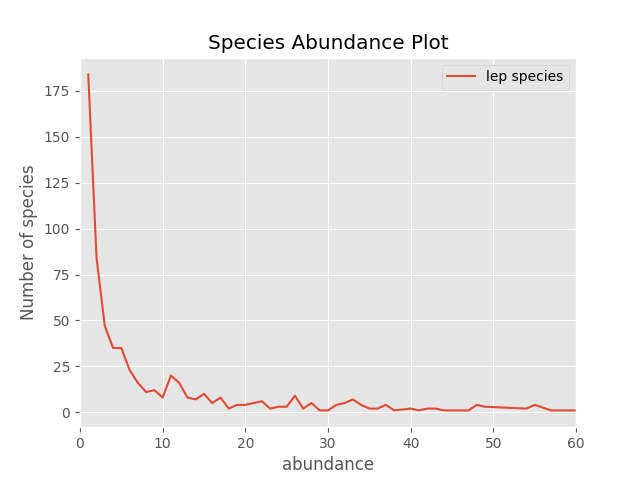
\includegraphics[width=800\linewidth,height=600\linewidth]{VPscripts/Species_vs_Abundance} \end{center}

\hypertarget{rank-abundance-plots}{%
\paragraph{Rank Abundance Plots}\label{rank-abundance-plots}}

These are another great way to visualize diversity. Again, rare species
are more commonly found. Common species are rarelky found. Higher ranks
are given to species with rare abundances.

\begin{Shaded}
\begin{Highlighting}[]
\CommentTok{\# Rank abundance plot : Relative abundancy vs. Rank (low rank is most abundant)}
\NormalTok{plt.figure()}
\NormalTok{spec\_rank }\OperatorTok{=}\NormalTok{ df2.sort\_values(}\StringTok{\textquotesingle{}abundance\textquotesingle{}}\NormalTok{, ascending}\OperatorTok{=}\VariableTok{False}\NormalTok{)}
\BuiltInTok{print}\NormalTok{(}\StringTok{"}\CharTok{\textbackslash{}n}\StringTok{Number of individuals: "}\NormalTok{, spec\_rank[}\StringTok{\textquotesingle{}abundance\textquotesingle{}}\NormalTok{].}\BuiltInTok{sum}\NormalTok{(), }\StringTok{"}\CharTok{\textbackslash{}n}\StringTok{"}\NormalTok{)}
\NormalTok{spec\_rank[}\StringTok{\textquotesingle{}abunprop\textquotesingle{}}\NormalTok{] }\OperatorTok{=}\NormalTok{ spec\_rank[}\StringTok{\textquotesingle{}abundance\textquotesingle{}}\NormalTok{]}\OperatorTok{/}\NormalTok{(spec\_rank[}\StringTok{\textquotesingle{}abundance\textquotesingle{}}\NormalTok{].}\BuiltInTok{sum}\NormalTok{())}
\NormalTok{spec\_rank[}\StringTok{\textquotesingle{}rank\textquotesingle{}}\NormalTok{] }\OperatorTok{=}\NormalTok{ spec\_rank.reset\_index().index }
\NormalTok{spec\_rank }\OperatorTok{=}\NormalTok{ spec\_rank.astype(\{}\StringTok{\textquotesingle{}abunprop\textquotesingle{}}\NormalTok{: }\BuiltInTok{float}\NormalTok{, }\StringTok{\textquotesingle{}rank\textquotesingle{}}\NormalTok{:}\BuiltInTok{int}\NormalTok{\})}
\NormalTok{spec\_rank[}\StringTok{\textquotesingle{}rank\textquotesingle{}}\NormalTok{] }\OperatorTok{+=}\DecValTok{1}
\NormalTok{spec\_rank[}\StringTok{\textquotesingle{}logabun\textquotesingle{}}\NormalTok{] }\OperatorTok{=}\NormalTok{ np.log(spec\_rank[}\StringTok{\textquotesingle{}abunprop\textquotesingle{}}\NormalTok{])}
\BuiltInTok{print}\NormalTok{(spec\_rank)}
\NormalTok{plt.scatter(spec\_rank[}\StringTok{\textquotesingle{}rank\textquotesingle{}}\NormalTok{], spec\_rank[}\StringTok{\textquotesingle{}logabun\textquotesingle{}}\NormalTok{], s }\OperatorTok{=} \FloatTok{0.5}\NormalTok{)}
\NormalTok{plt.savefig(}\StringTok{\textquotesingle{}Rank Abundance.png\textquotesingle{}}\NormalTok{)}
\end{Highlighting}
\end{Shaded}

\begin{center}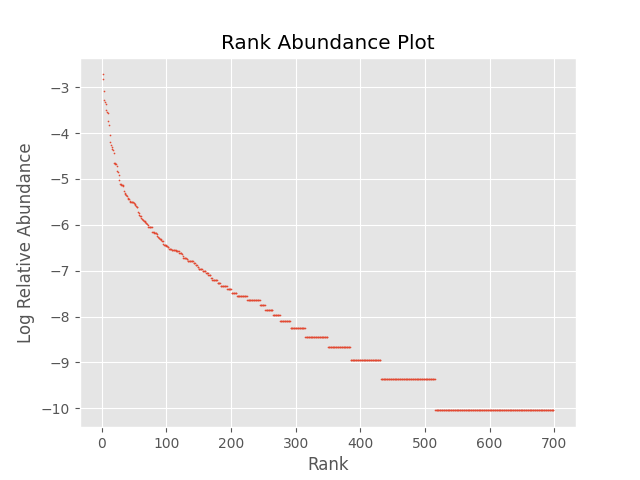
\includegraphics[width=800\linewidth,height=600\linewidth]{VPscripts/Rank Abundance} \end{center}

\hypertarget{diet-breadth-data-what-i-was-after}{%
\paragraph{Diet Breadth data (what I was
after!)}\label{diet-breadth-data-what-i-was-after}}

One of my research interests is the evolution of specialization; we
observe countless instances of specialization in host
plant-caterpillar-parasitoid systems. I would love to continue the work
documenting the interactions in these systems and give power to the data
that people hve collected long term. Here's an attempt to visualize host
plant specialization.

\begin{Shaded}
\begin{Highlighting}[]
\CommentTok{\#Diet breadth, all instances of host plants recorded for each species }
\NormalTok{diet\_names }\OperatorTok{=}\NormalTok{ df.groupby(}\StringTok{\textquotesingle{}lep species\textquotesingle{}}\NormalTok{)[}\StringTok{\textquotesingle{}plant species\textquotesingle{}}\NormalTok{].unique()}
\NormalTok{diet\_names.to\_csv(}\StringTok{"names\_diet.csv"}\NormalTok{)}
\NormalTok{diet\_number }\OperatorTok{=}\NormalTok{ df.groupby(}\StringTok{\textquotesingle{}lep species\textquotesingle{}}\NormalTok{)[}\StringTok{\textquotesingle{}plant species\textquotesingle{}}\NormalTok{].nunique()}
\NormalTok{diet\_number.to\_csv(}\StringTok{"numbers\_diet.csv"}\NormalTok{)}
\NormalTok{df\_names }\OperatorTok{=}\NormalTok{ pd.read\_csv(}\StringTok{"names\_diet.csv"}\NormalTok{)}
\NormalTok{df\_num }\OperatorTok{=}\NormalTok{ pd.read\_csv(}\StringTok{"numbers\_diet.csv"}\NormalTok{)}
\NormalTok{diet\_full }\OperatorTok{=}\NormalTok{ pd.merge(df\_names, df\_num, on}\OperatorTok{=}\StringTok{\textquotesingle{}lep species\textquotesingle{}}\NormalTok{)}
\NormalTok{diet\_full.to\_csv(}\StringTok{"Diet Breadth Summary.csv"}\NormalTok{)}
\end{Highlighting}
\end{Shaded}

\begin{Shaded}
\begin{Highlighting}[]
\NormalTok{diet\_breadth\_num }\OtherTok{=} \FunctionTok{read.csv}\NormalTok{(}\StringTok{"VPscripts/Diet Breadth Summary.csv"}\NormalTok{)}
\FunctionTok{head}\NormalTok{(diet\_breadth\_num)}
\end{Highlighting}
\end{Shaded}

\begin{verbatim}
##   X       lep.species plant.species_x
## 1 0   acharia horrida               1
## 2 1 acharia hyperoche               2
## 3 2     acharia nesea               8
## 4 3 acharia ophelians               1
## 5 4    acharia sarans               8
## 6 5        acharia sp               3
##                                                                                                                                                        plant.species_y
## 1                                                                                                                                             ['calathea crotalifera']
## 2                                                                                                                                  ['musa acuminata' nan 'solanum sp']
## 3 ['anthurium sp' nan 'hyeronima alchorneoides' 'inga edulis' 'heliconia sp'\n 'anthurium clavigerum' 'piper reticulatum' 'guatteria diospyroides'\n 'adelia triloba']
## 4                                                                                                                                                     ['heliconia sp']
## 5               [nan 'alchornea costaricensis' 'musa sp' 'heliconia sp'\n 'anthurium clavigerum' 'neea psychotroides' 'calathea lutea'\n 'anthurium sp' 'calathea sp']
## 6                                                                                                                        ['piper colonense' 'piper sp' 'heliconia sp']
\end{verbatim}

\begin{Shaded}
\begin{Highlighting}[]
\NormalTok{plt.figure()}
\NormalTok{breadth }\OperatorTok{=}\NormalTok{ df\_num.groupby(}\StringTok{\textquotesingle{}plant species\textquotesingle{}}\NormalTok{)[}\StringTok{\textquotesingle{}lep species\textquotesingle{}}\NormalTok{].count().plot()}
\NormalTok{plt.xlabel(}\StringTok{"Diet {-} \# of host plant species"}\NormalTok{)}
\NormalTok{plt.ylabel(}\StringTok{"Number of Lepidopteran Species"}\NormalTok{)}
\NormalTok{plt.title(}\StringTok{"Diet Breadth Plot"}\NormalTok{)}
\NormalTok{plt.savefig(}\StringTok{"Diet Breadth Plot"}\NormalTok{)}
\end{Highlighting}
\end{Shaded}

\begin{center}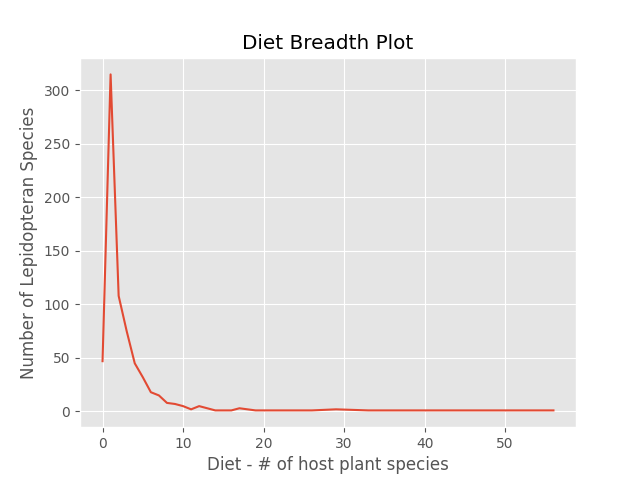
\includegraphics[width=800\linewidth,height=600\linewidth]{VPscripts/Diet Breadth Plot} \end{center}

\hypertarget{future-goals-1}{%
\paragraph{Future Goals}\label{future-goals-1}}

\begin{itemize}
\tightlist
\item
  Visualizing beta, gamma, interaction diversity\\
\item
  Importing virus data to observe infection rates across taxa
\item
  Importing parasitoid data to observe parasitism rates across taxa
\item
  Combining data from 3 sites to show latitudinal, or at least
  geographic, variation
\end{itemize}

\end{document}
